% =====================================================================
% LATEX CODE SNIPPETS FOR INCLUDING DIAGRAMS IN YOUR IEEE PAPER
% Copy and paste these into your IEEE_PAPER.tex file
% =====================================================================

% =====================================================================
% SECTION III: SYSTEM ARCHITECTURE
% Place this where you have "Figure 1 should go here"
% =====================================================================

\begin{figure*}[htbp]
\centerline{\includegraphics[width=\textwidth]{research-diagrams/system_architecture.pdf}}
\caption{Three-tier architecture of the AI-powered virtual legal assistant system showing frontend (Next.js), backend (Express.js), and AI service (Python) layers with core components including local embedding model, FAISS vector database, and Gemini LLM.}
\label{fig:system_architecture}
\end{figure*}

% Reference in text: As shown in Fig.~\ref{fig:system_architecture}, the system...

% =====================================================================
% SECTION IV: RAG WORKFLOW
% =====================================================================

\begin{figure*}[htbp]
\centerline{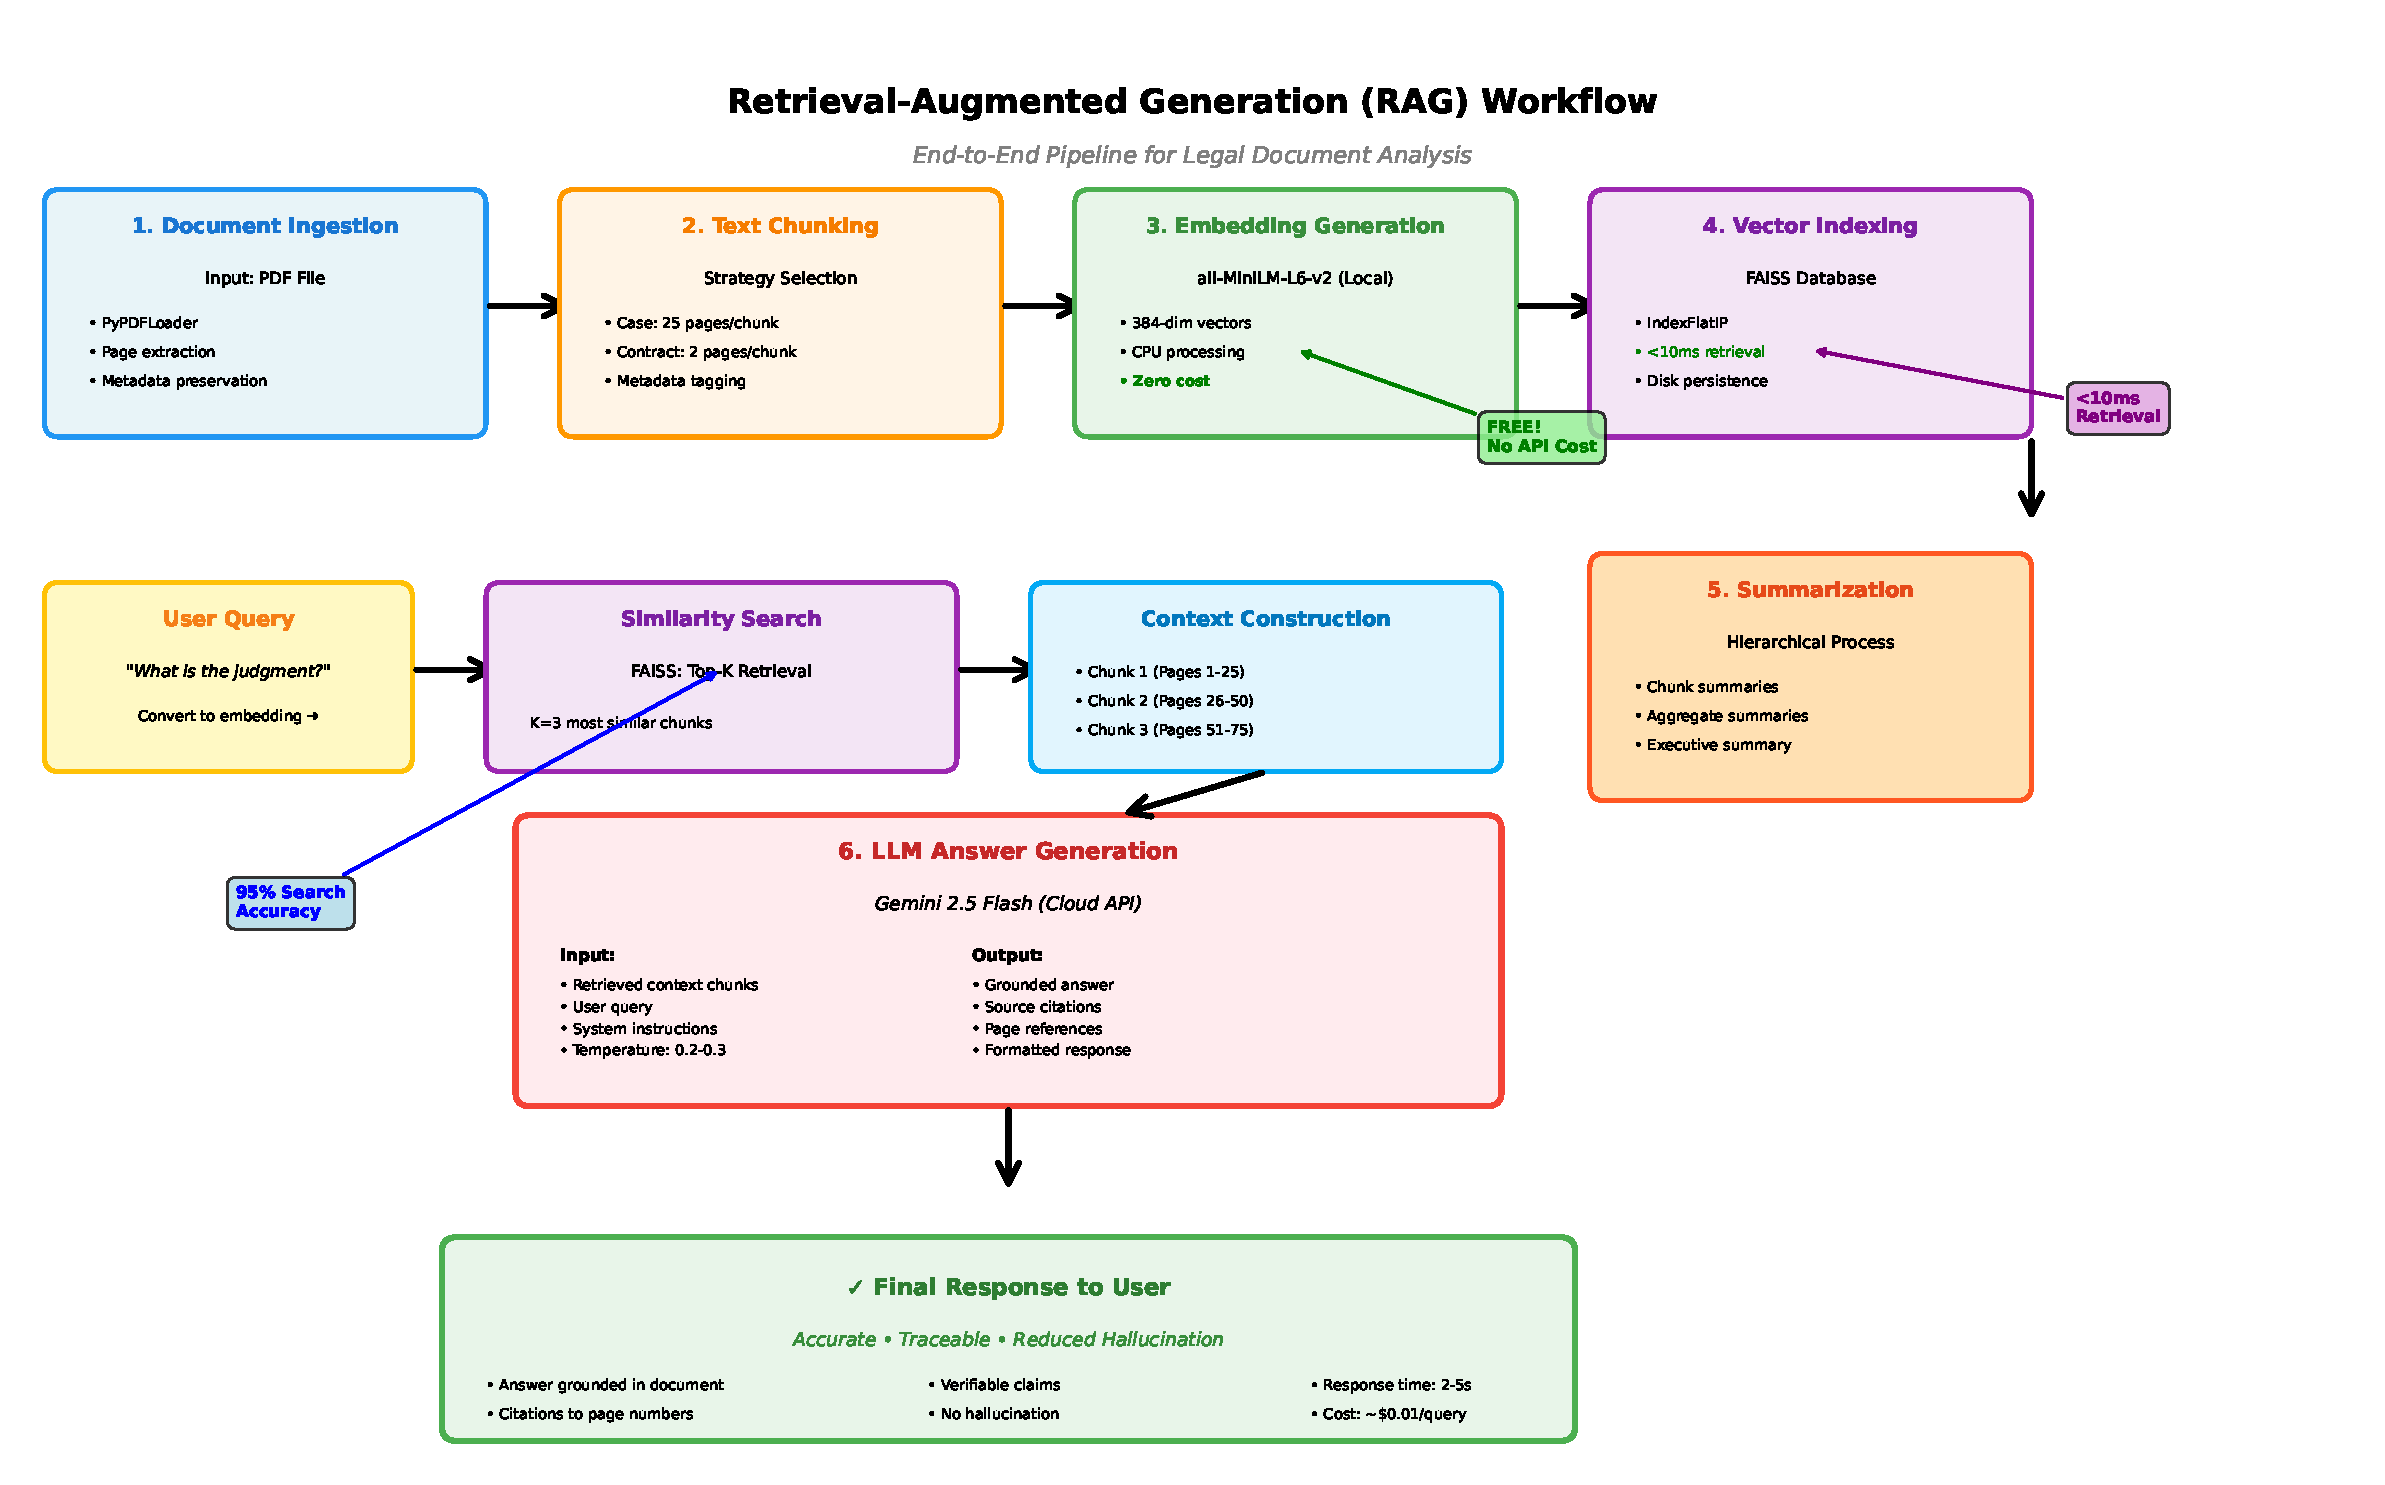
\includegraphics[width=\textwidth]{research-diagrams/rag_workflow.pdf}}
\caption{Complete Retrieval-Augmented Generation (RAG) workflow showing the six-stage pipeline: (1) document ingestion, (2) text chunking, (3) embedding generation using all-MiniLM-L6-v2, (4) FAISS vector indexing, (5) similarity search with top-K retrieval, and (6) LLM-based answer generation with source citations.}
\label{fig:rag_workflow}
\end{figure*}

% Reference in text: The RAG workflow (Fig.~\ref{fig:rag_workflow}) demonstrates...

% =====================================================================
% SECTION III: DATA FLOW (Optional - use if you want to show the flow)
% =====================================================================

\begin{figure*}[htbp]
\centerline{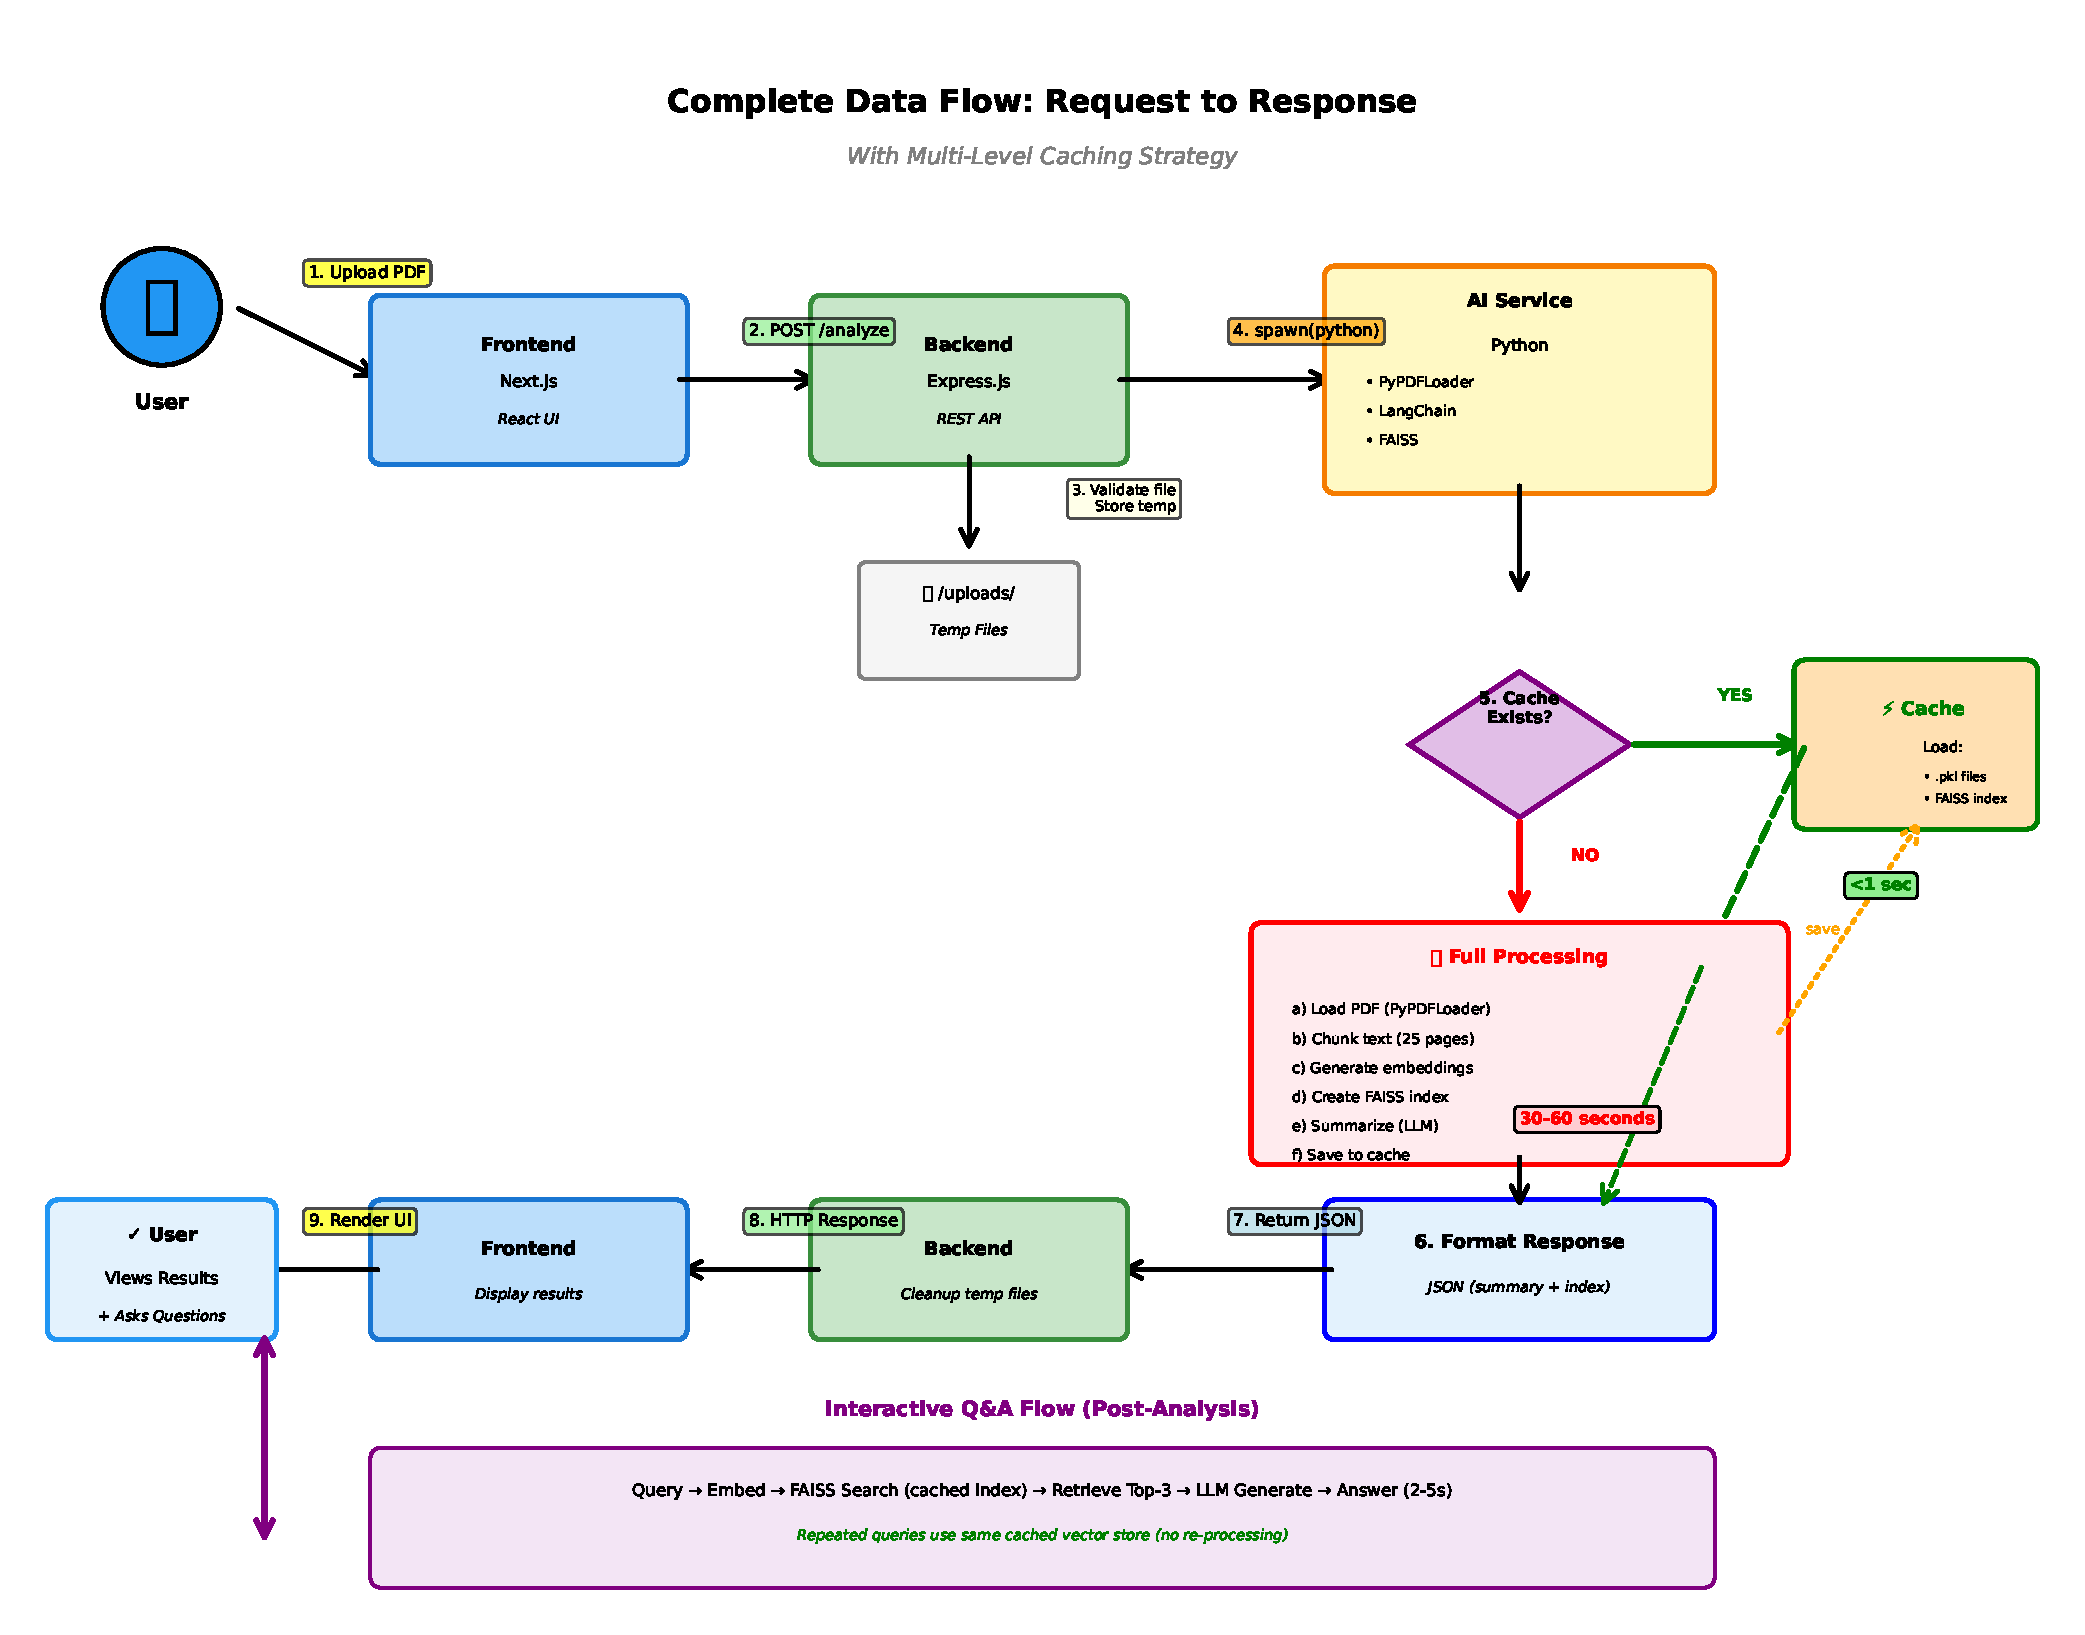
\includegraphics[width=0.9\textwidth]{research-diagrams/data_flow_diagram.pdf}}
\caption{Complete data flow from user request to response, illustrating the multi-level caching strategy. Cache hits achieve sub-second response times while cache misses require 30-60 seconds for full document processing. The Q\&A mode leverages cached vector stores for 2-5 second query responses.}
\label{fig:data_flow}
\end{figure*}

% Reference in text: The data flow (Fig.~\ref{fig:data_flow}) shows...

% =====================================================================
% SECTION V: CASE ANALYSIS WORKFLOW
% =====================================================================

\begin{figure}[htbp]
\centerline{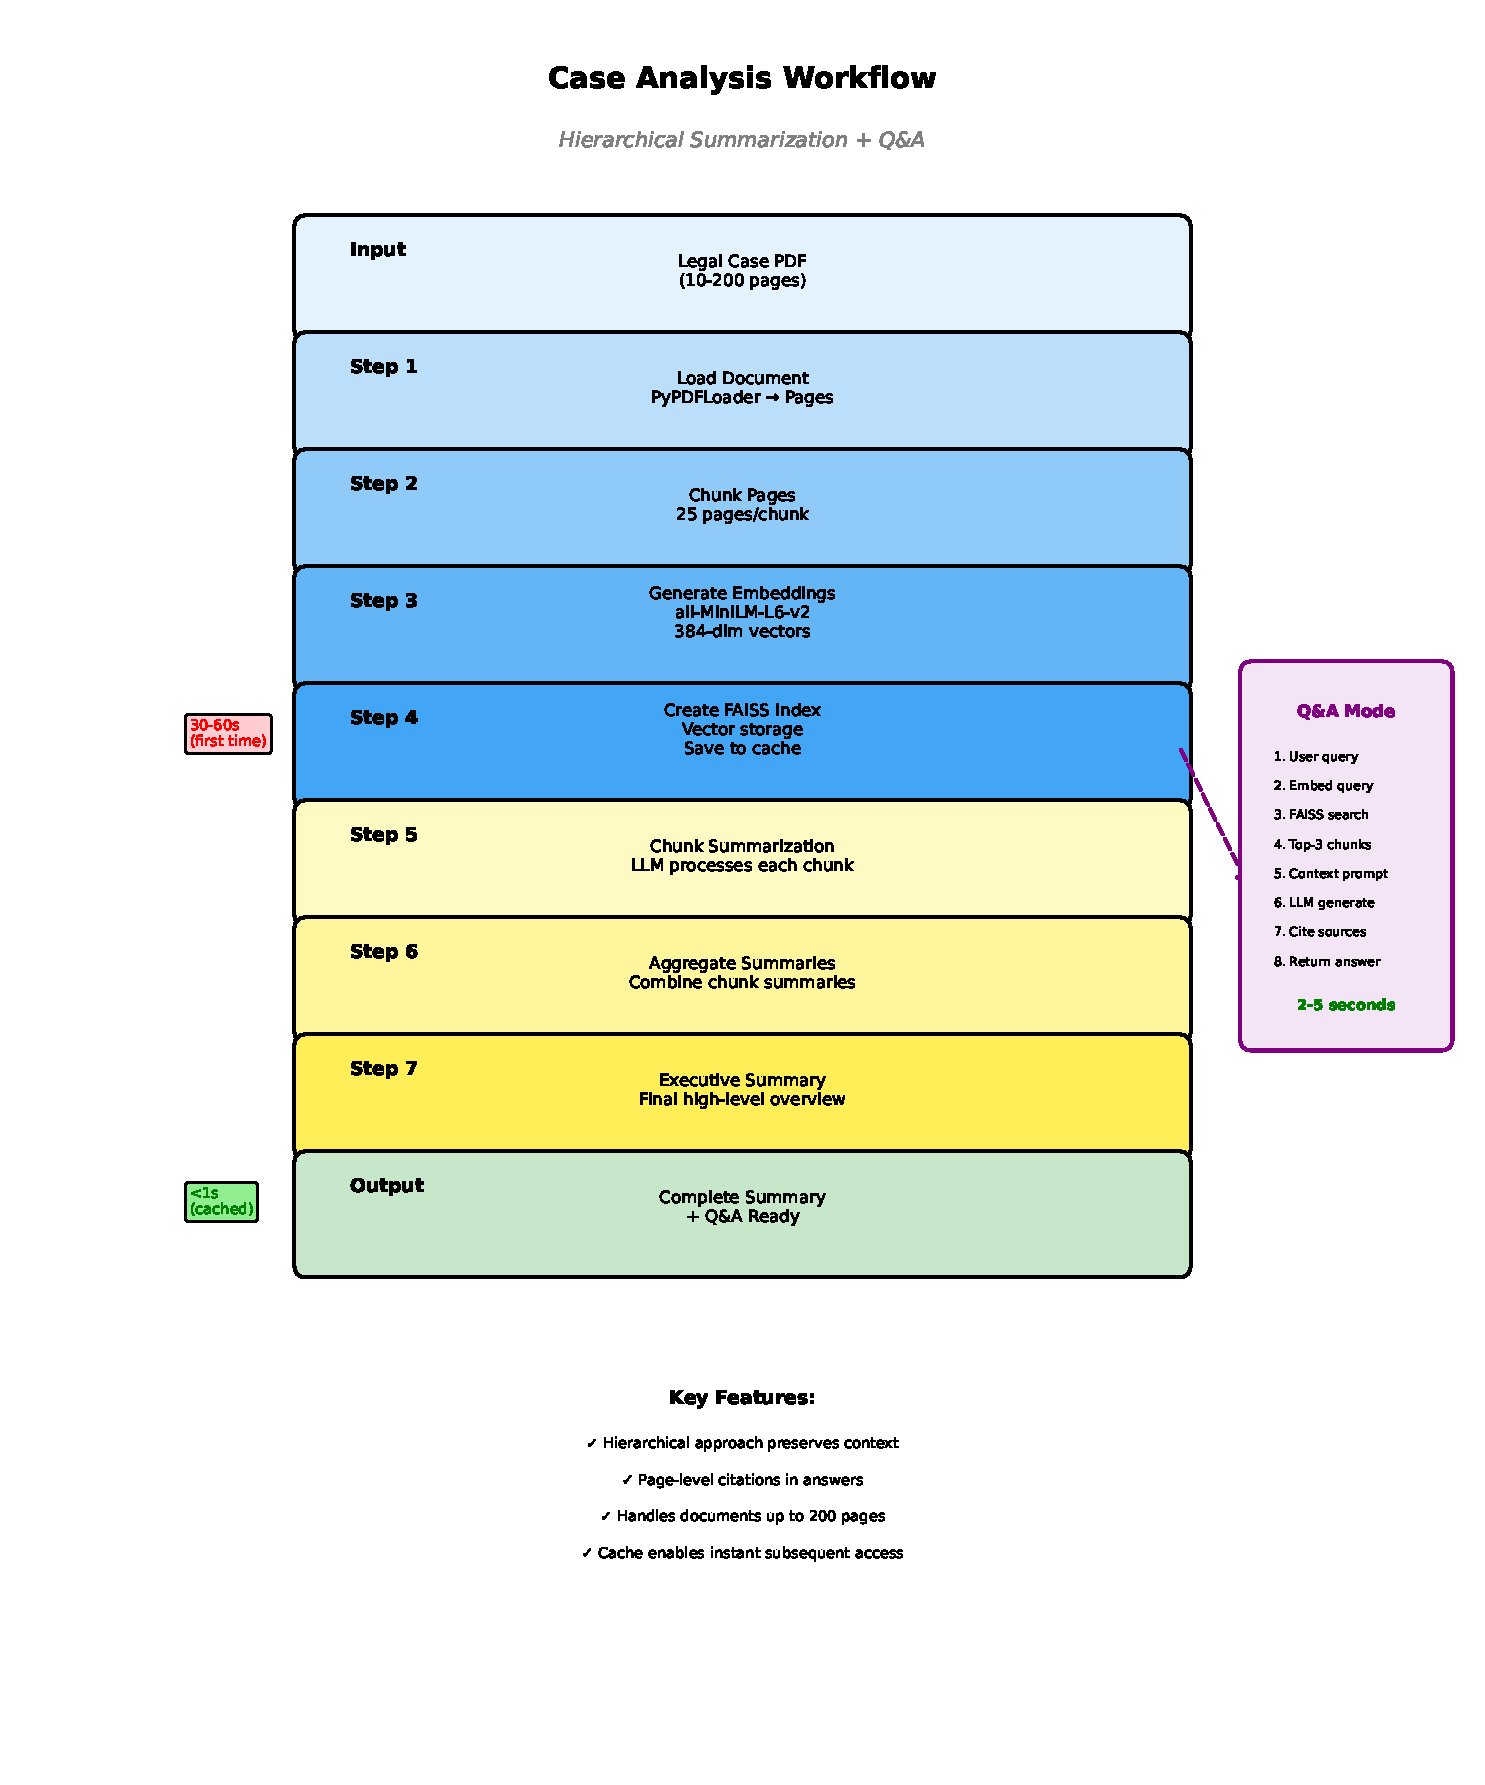
\includegraphics[width=\columnwidth]{research-diagrams/flow_case_analysis.pdf}}
\caption{Case analysis workflow showing hierarchical summarization approach with 25-page chunking strategy. The process includes document loading, embedding generation, FAISS indexing, and multi-level summarization to produce executive summaries with interactive Q\&A capability.}
\label{fig:case_analysis}
\end{figure}

% Reference in text: The case analysis workflow (Fig.~\ref{fig:case_analysis})...

% =====================================================================
% SECTION V: CONTRACT ANALYSIS WORKFLOW
% =====================================================================

\begin{figure}[htbp]
\centerline{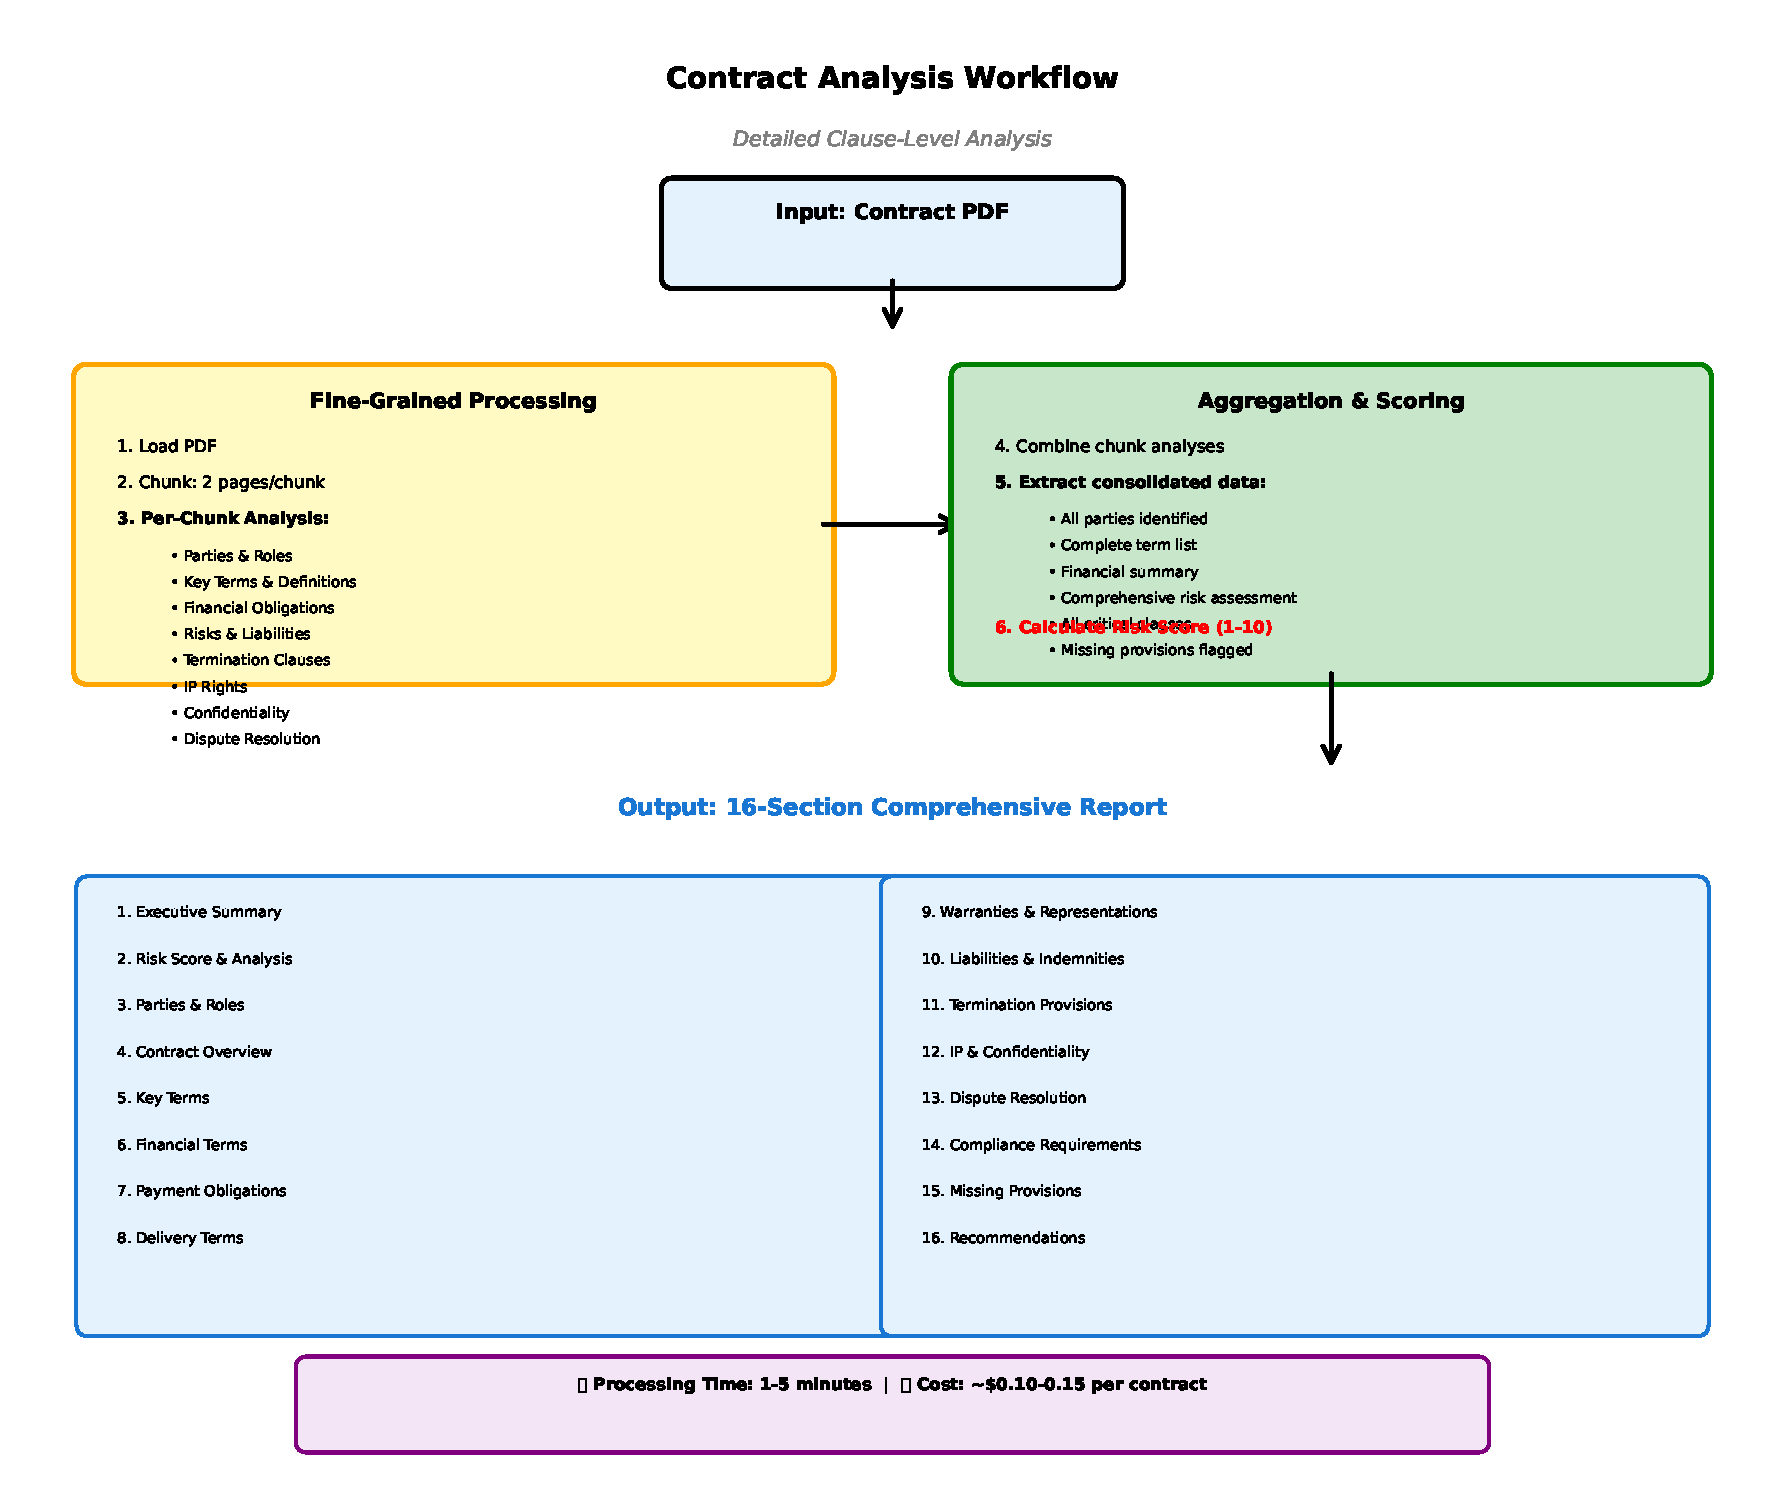
\includegraphics[width=\columnwidth]{research-diagrams/flow_contract_analysis.pdf}}
\caption{Contract analysis workflow with fine-grained 2-page chunking for detailed clause-level extraction. The system analyzes 16 distinct sections including parties, terms, risks, liabilities, and compliance requirements, generating a comprehensive report with risk scoring.}
\label{fig:contract_analysis}
\end{figure}

% Reference in text: For contract analysis (Fig.~\ref{fig:contract_analysis})...

% =====================================================================
% SECTION VI: PERFORMANCE METRICS TABLE
% Place this in Results section
% =====================================================================

\begin{table}[htbp]
\caption{System Performance Metrics}
\begin{center}
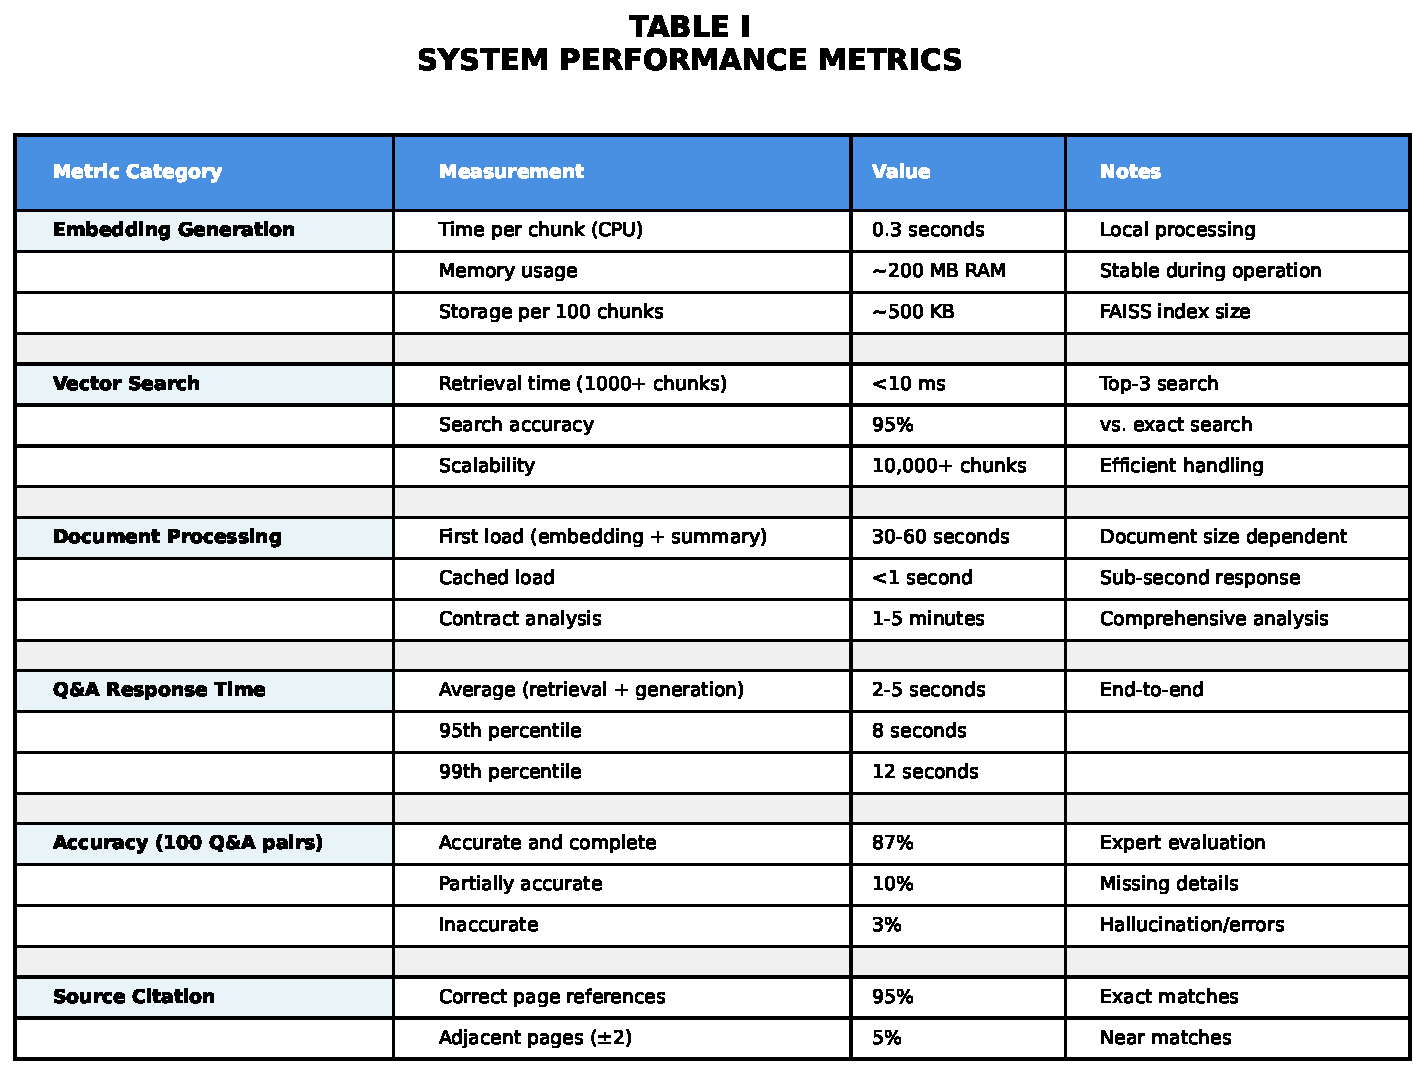
\includegraphics[width=\columnwidth]{research-diagrams/table_performance_metrics.pdf}
\end{center}
\label{table:performance}
\end{table}

% Alternative if you want it as a figure:
% \begin{figure}[htbp]
% \centerline{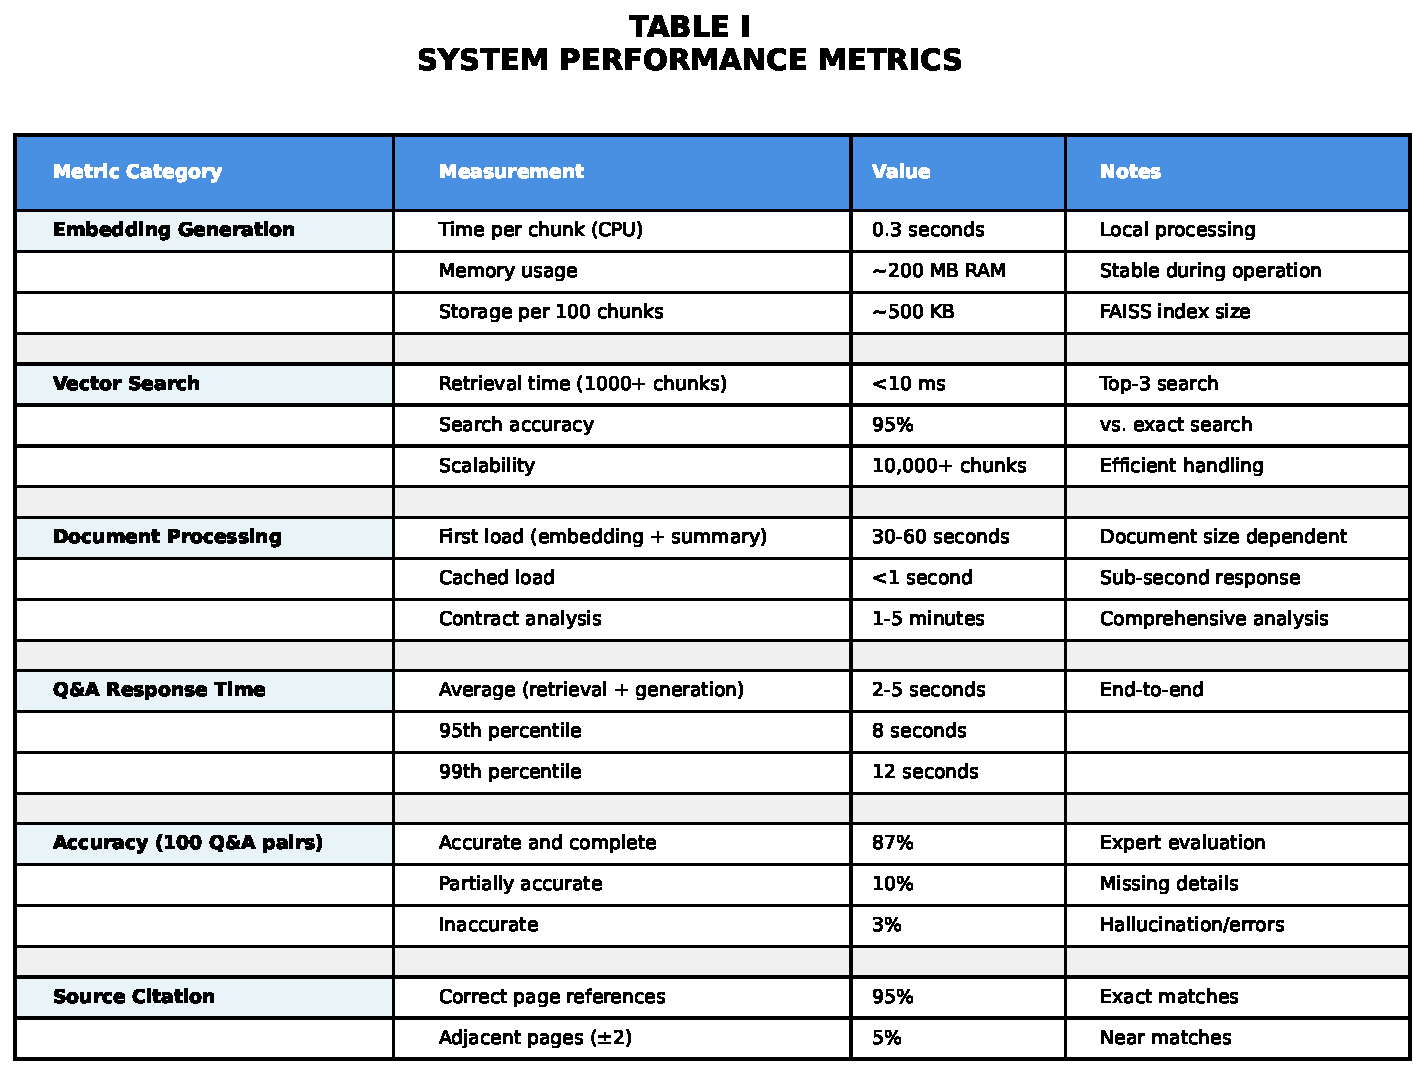
\includegraphics[width=\columnwidth]{research-diagrams/table_performance_metrics.pdf}}
% \caption{System Performance Metrics across embedding generation, vector search, document processing, Q\&A response times, and accuracy evaluation.}
% \label{table:performance}
% \end{figure}

% =====================================================================
% SECTION VI: RAG VS STANDALONE LLM COMPARISON
% =====================================================================

\begin{table}[htbp]
\caption{RAG vs Standalone LLM Comparison}
\begin{center}
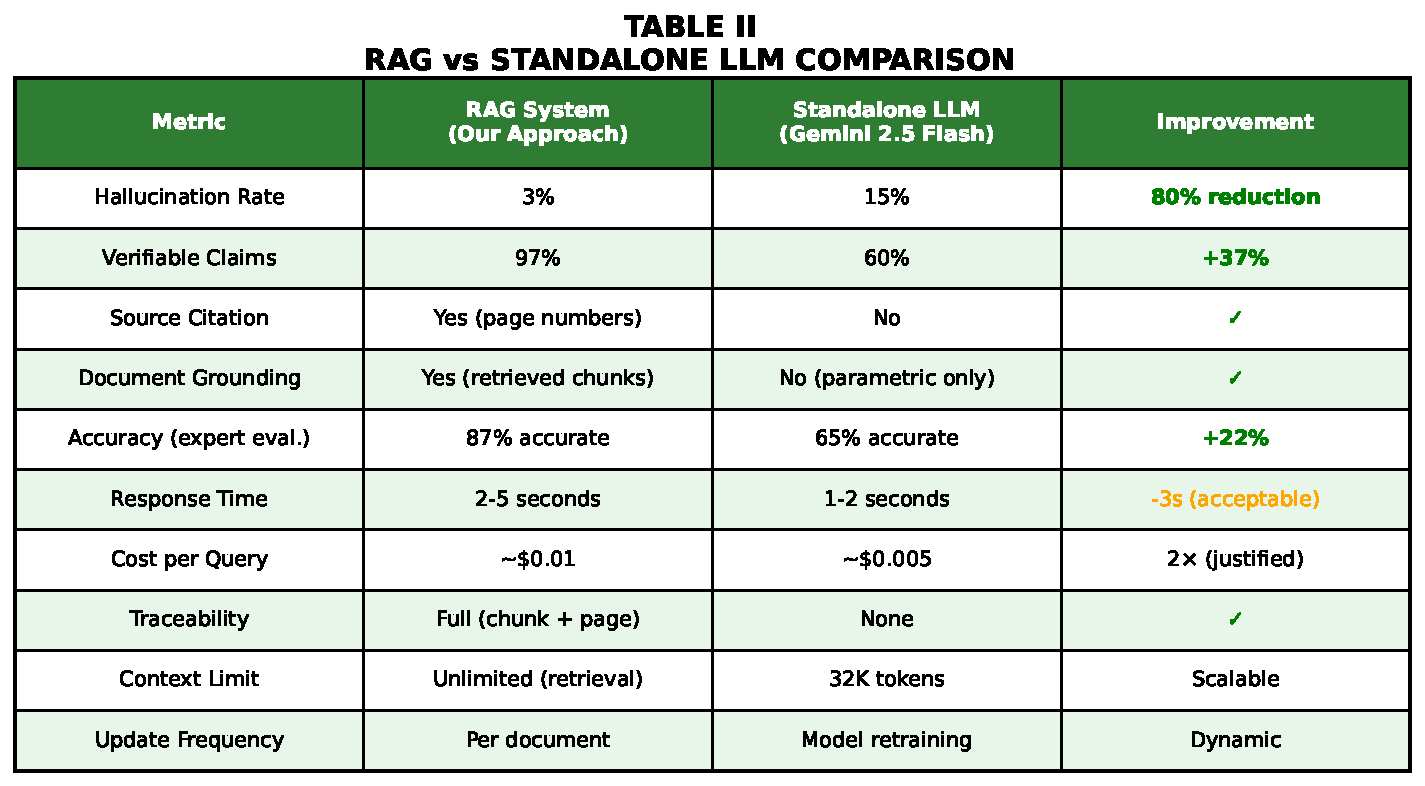
\includegraphics[width=\columnwidth]{research-diagrams/table_rag_comparison.pdf}
\end{center}
\label{table:rag_comparison}
\end{table}

% Reference in text: Table~\ref{table:rag_comparison} demonstrates the superiority...

% =====================================================================
% SECTION VI: COST ANALYSIS TABLE
% =====================================================================

\begin{table}[htbp]
\caption{Cost Analysis: Traditional vs Local Embeddings Approach}
\begin{center}
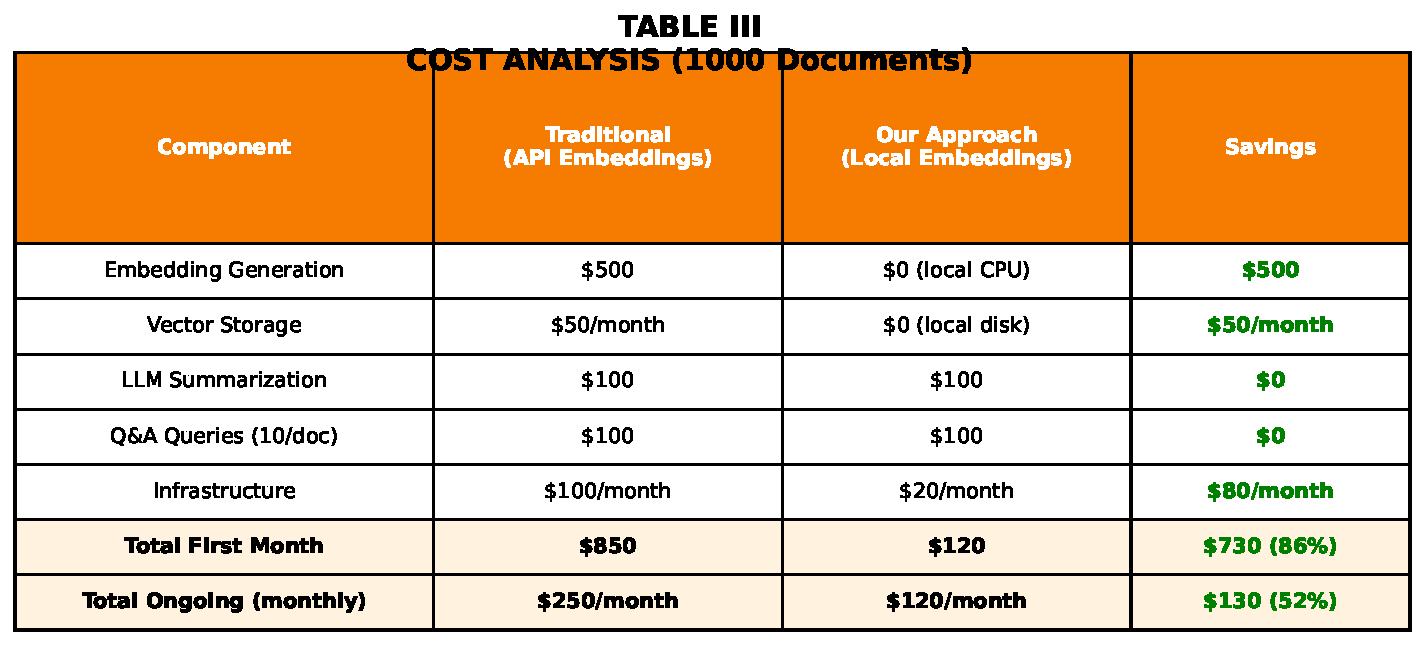
\includegraphics[width=\columnwidth]{research-diagrams/table_cost_analysis.pdf}
\end{center}
\label{table:cost_analysis}
\end{table}

% Reference in text: Our cost analysis (Table~\ref{table:cost_analysis}) shows...

% =====================================================================
% TIPS FOR USING THESE FIGURES
% =====================================================================

% 1. figure* spans both columns in IEEE two-column format
% 2. figure fits in single column
% 3. Use \textwidth for figure* and \columnwidth for figure
% 4. Always use PDF files for best quality (vector graphics)
% 5. Reference figures using \ref{label_name}
% 6. Place figures near where they're first mentioned
% 7. Use [htbp] for placement: h=here, t=top, b=bottom, p=page

% =====================================================================
% ALTERNATIVE: IF YOU WANT TO USE PNG INSTEAD OF PDF
% =====================================================================

% Just replace .pdf with .png in all \includegraphics commands:
% 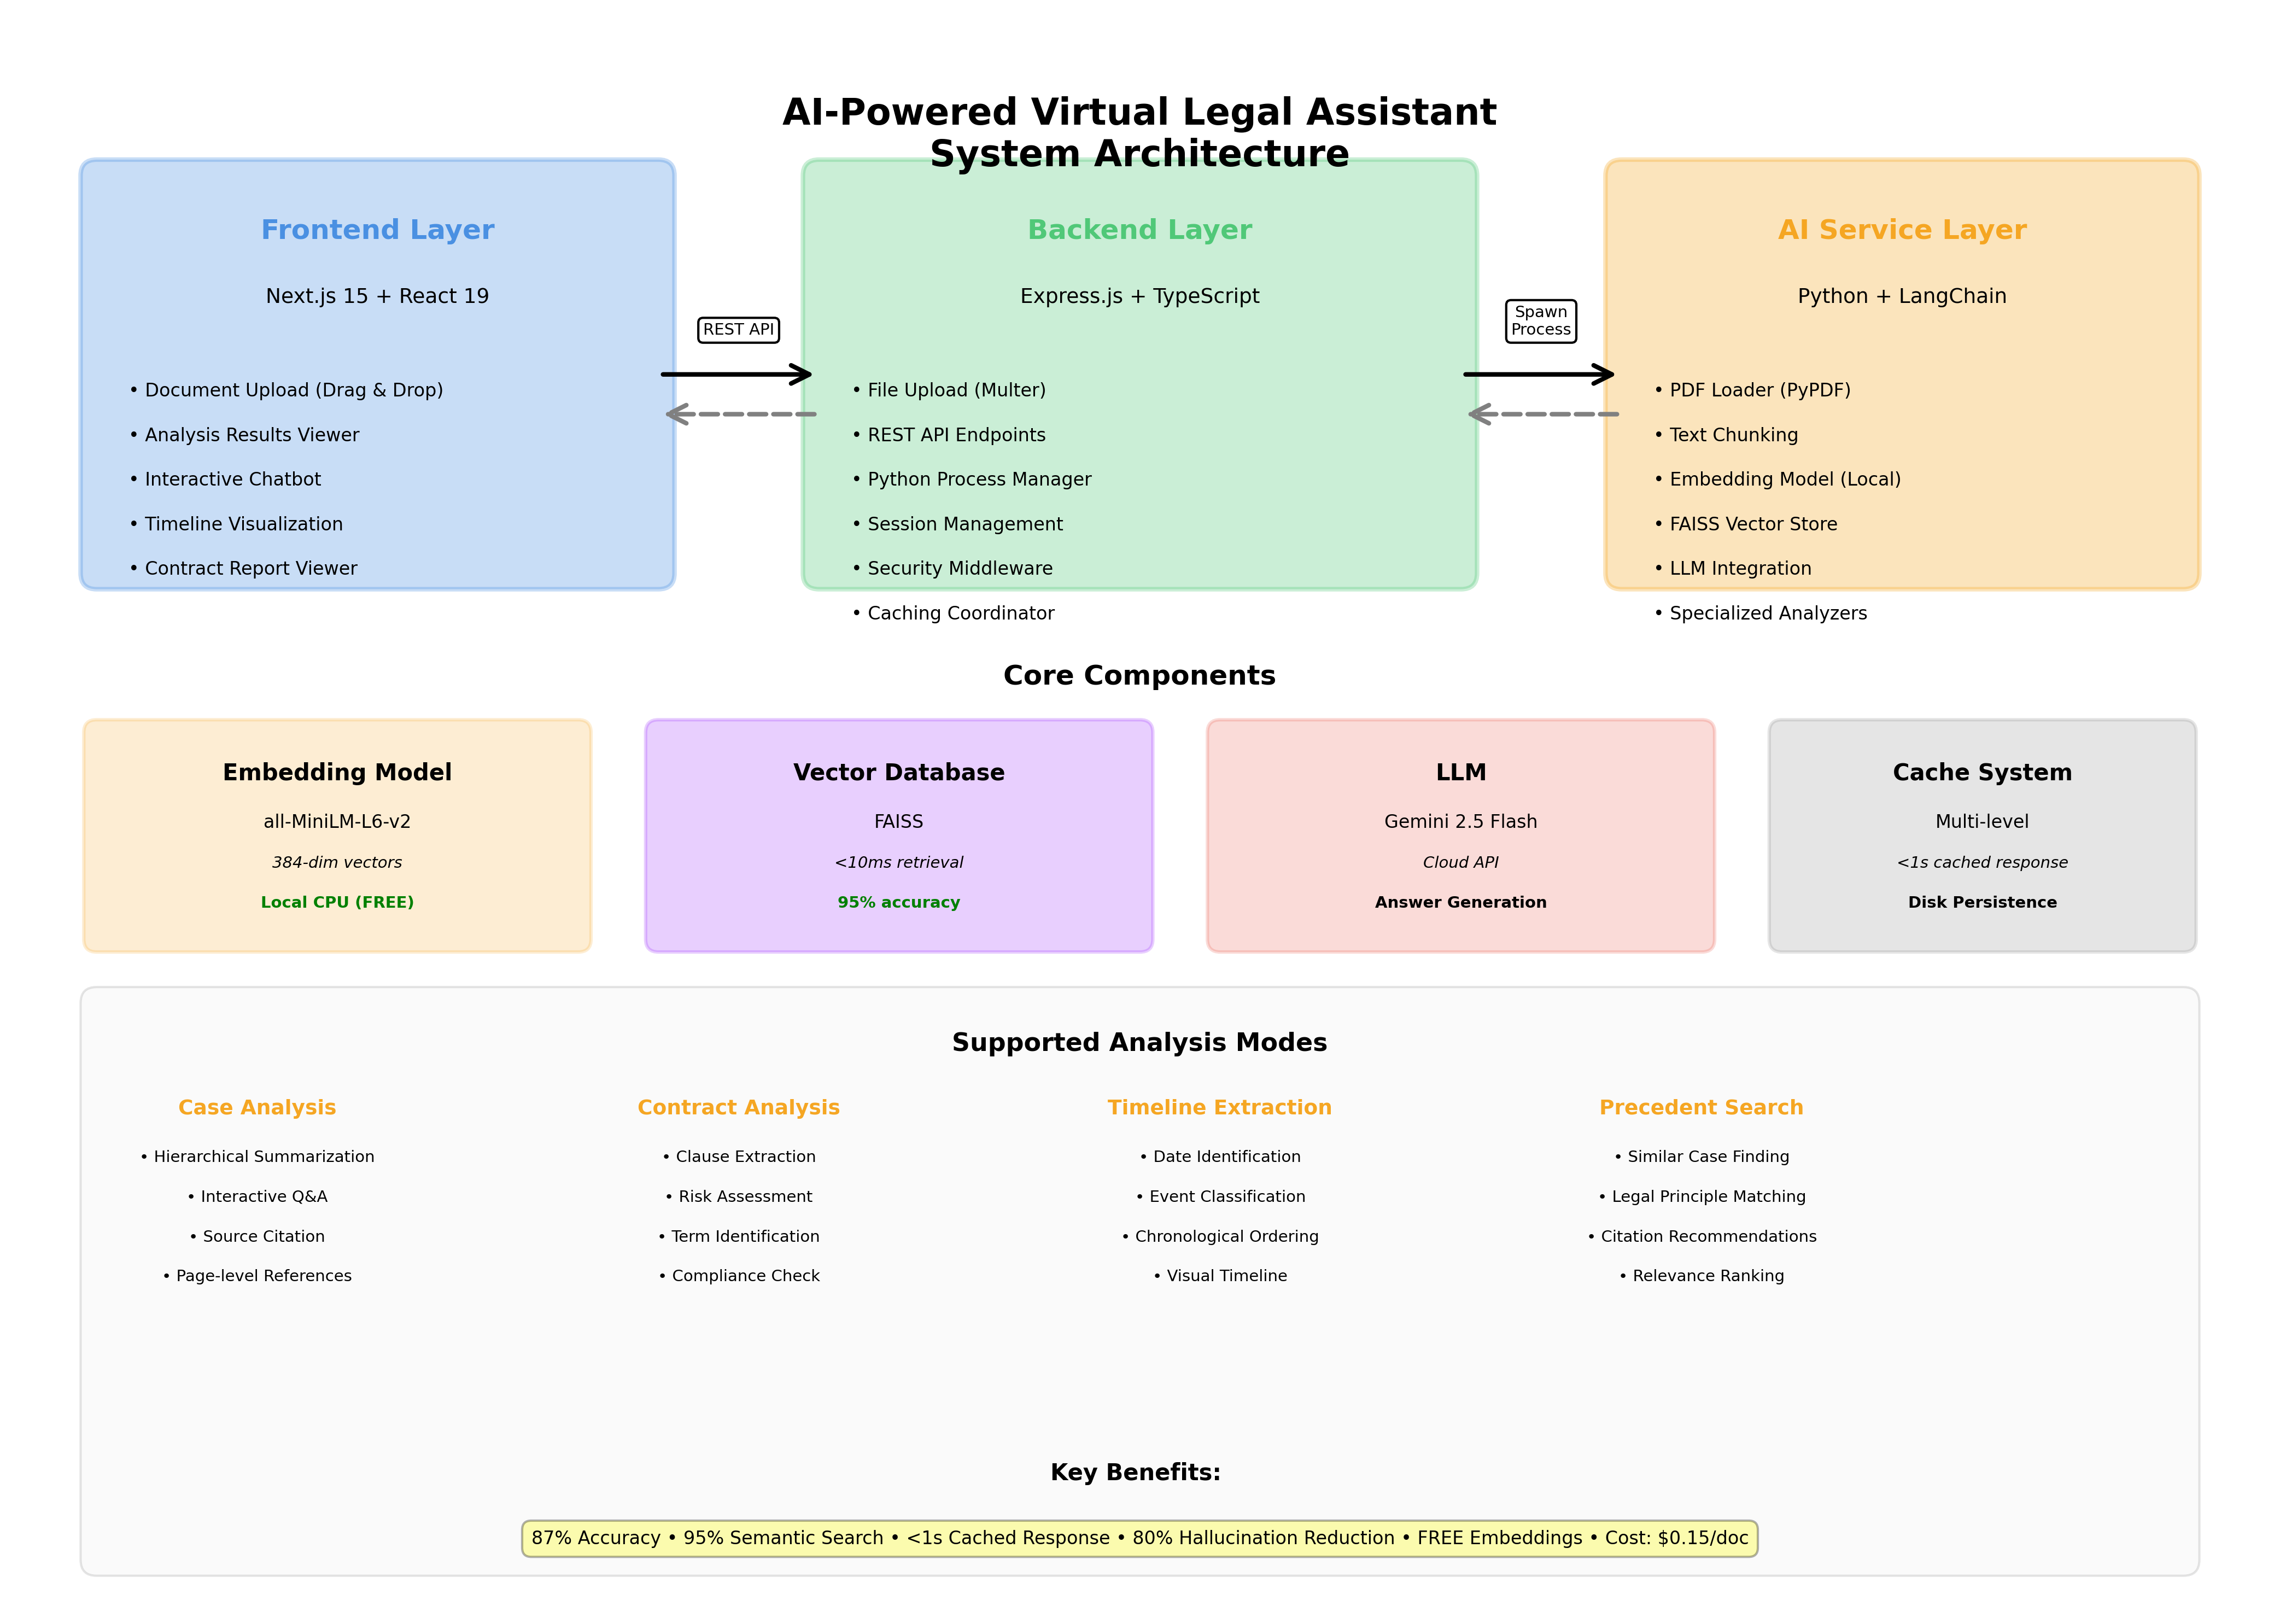
\includegraphics[width=\columnwidth]{research-diagrams/system_architecture.png}

% However, PDF is recommended for publications (vector graphics scale better)

% =====================================================================
% CROSS-REFERENCING IN TEXT
% =====================================================================

% Use these patterns in your text:
% - "as shown in Fig.~\ref{fig:system_architecture}"
% - "the RAG workflow (Fig.~\ref{fig:rag_workflow})"
% - "Table~\ref{table:performance} presents"
% - "see Fig.~\ref{fig:data_flow} for details"

% The ~ creates a non-breaking space between "Fig." and the number

% =====================================================================
% RECOMMENDED PLACEMENT IN YOUR PAPER
% =====================================================================

% Section III (System Architecture):
%   - Fig. 1: system_architecture.pdf (full width, figure*)
%   - Fig. 2: data_flow_diagram.pdf (optional, full width)

% Section IV (RAG Workflow):
%   - Fig. 3: rag_workflow.pdf (full width, figure*)

% Section V (Methodology):
%   - Fig. 4: flow_case_analysis.pdf (single column)
%   - Fig. 5: flow_contract_analysis.pdf (single column)

% Section VI (Results):
%   - Table I: table_performance_metrics.pdf
%   - Table II: table_rag_comparison.pdf
%   - Table III: table_cost_analysis.pdf

% =====================================================================
% COMPILATION
% =====================================================================

% Make sure research-diagrams folder is in the same directory as your .tex file
% Or use relative/absolute paths:
% \includegraphics[width=\columnwidth]{../research-diagrams/system_architecture.pdf}

% Compile with:
% pdflatex IEEE_PAPER.tex
% bibtex IEEE_PAPER
% pdflatex IEEE_PAPER.tex
% pdflatex IEEE_PAPER.tex

% =====================================================================
